\section{Model}

Firstly the models are determined for the lower frequency bands:
\begin{enumerate}
\item 33 Hz to 66 Hz
\item 66 Hz to 132 Hz
\item 132 Hz to 265 Hz
\item 265 Hz to 530 Hz,
\end{enumerate}
Are created. The models are based on experiments documented in \autoref{app:journal_speaker_test3}. The model depicted in \autoref{fig:combineModelreport} shows how THD increases according to the RMS value. 


\begin{figure}[H]
    \centering
    \tikzsetnextfilename{BandModelCombineReport}
    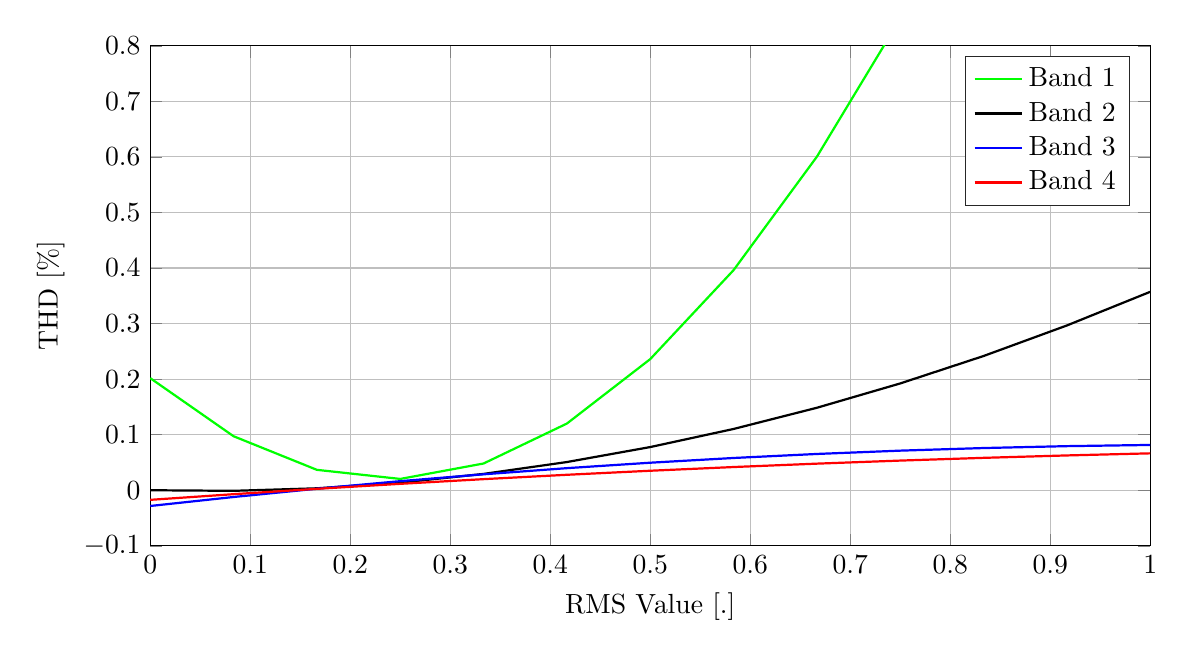
\begin{tikzpicture}

\begin{axis}[%
width=5.0in,
height=2.5in,
at={(0.758in,0.481in)},
scale only axis,
xmin=0,
xmax=1,
xmajorgrids,
ymajorgrids,
xlabel={RMS Value [.]},
ymin=-0.1,
ymax=0.8,
ylabel={THD [\%]},
ytick={-0.1, 0, 0.1,  0.2,  0.3, 0.4, 0.5, 0.6, 0.7, 0.8},
axis background/.style={fill=white},
legend style={legend cell align=left,align=left,draw=white!15!black}
%every axis legend/.code={\let\addlegendentry\relax}
]
\addplot [color=green,solid,thick]
  table[row sep=crcr]{%
0	0.2018\\
0.0833333333333333	0.0971958333333334\\
0.166666666666667	0.0367166666666667\\
0.25	0.0203625\\
0.333333333333333	0.0481333333333334\\
0.416666666666667	0.120029166666667\\
0.5	0.23605\\
0.583333333333333	0.396195833333334\\
0.666666666666667	0.600466666666667\\
0.75	0.8488625\\
0.833333333333333	1.14138333333333\\
0.916666666666667	1.47802916666667\\
1	1.8588\\
};
\addlegendentry{Band 1};


\addplot [color=black,solid,thick]
  table[row sep=crcr]{%
0	0\\
0.0833333333333333	-0.00105625\\
0.166666666666667	0.00349166666666667\\
0.25	0.01364375\\
0.333333333333333	0.0294\\
0.416666666666667	0.0507604166666667\\
0.5	0.077725\\
0.583333333333333	0.11029375\\
0.666666666666667	0.148466666666667\\
0.75	0.19224375\\
0.833333333333333	0.241625\\
0.916666666666667	0.296610416666667\\
1	0.3572\\
};
\addlegendentry{Band 2};

\addplot [color=blue,solid,thick]
  table[row sep=crcr]{%
0	-0.02834\\
0.0833333333333333	-0.0121695138888889\\
0.166666666666667	0.00272527777777777\\
0.25	0.016344375\\
0.333333333333333	0.0286877777777778\\
0.416666666666667	0.0397554861111111\\
0.5	0.0495475\\
0.583333333333333	0.0580638194444444\\
0.666666666666667	0.0653044444444444\\
0.75	0.071269375\\
0.833333333333333	0.0759586111111111\\
0.916666666666667	0.0793721527777778\\
1	0.08151\\
};
\addlegendentry{Band 3};

\addplot [color=red,solid,thick]
  table[row sep=crcr]{%
0	-0.01729\\
0.0833333333333333	-0.00709902777777778\\
0.166666666666667	0.00250722222222222\\
0.25	0.01152875\\
0.333333333333333	0.0199655555555556\\
0.416666666666667	0.0278176388888889\\
0.5	0.035085\\
0.583333333333333	0.0417676388888889\\
0.666666666666667	0.0478655555555556\\
0.75	0.05337875\\
0.833333333333333	0.0583072222222222\\
0.916666666666667	0.0626509722222222\\
1	0.06641\\
};
\addlegendentry{Band 4};

\end{axis}
\end{tikzpicture}
    \caption{4 Interpolated model describing the worst case THD in each band. Further described in \autoref{app:app:journal_speaker_test3}}
    \label{fig:CombinedModelreport}
\end{figure}

\autoref{fig:combineModelreport}